\mode*

\section{Vad är en fil?}

\begin{frame}
  \begin{definition}<1,3>[Primärminne]
    \begin{itemize}
      \item Datorns arbetsminne.
      \item Exekverande program (processer) och data (variabler) lagras här.
      \item Flyktigt minne.
      \item Snabbt: storleksordning nanosekunder.
    \end{itemize}
  \end{definition}

  \begin{definition}<2,3>[Sekundärminne]
    \begin{itemize}
      \item Långsammare minne: storleksordning mikro- till millisekunder.
      \item Oflyktigt.
      \item Icke-exekverande program och data (filer) lagras här.
    \end{itemize}
  \end{definition}
\end{frame}

\begin{frame}
  \begin{block}{Filer}
    \begin{itemize}
      \item Vi har erfarenhet av filer.
      \item Våra program är sparade i filer.
    \end{itemize}
  \end{block}

  \pause

  \begin{example}
    \begin{itemize}
      \item Pythonprogram,
      \item bilder,
      \item dokument,
      \item \etc
    \end{itemize}
  \end{example}
\end{frame}

\begin{frame}
  \begin{remark}
    \begin{itemize}
      \item Behövs för att minnas mellan körningarna.
      \item Behövs för att överföra data mellan program.
      \item Behövs för att hantera kopiösa mängder data.
    \end{itemize}
  \end{remark}
\end{frame}


\section{Hur använder vi filer?}

\begin{frame}
  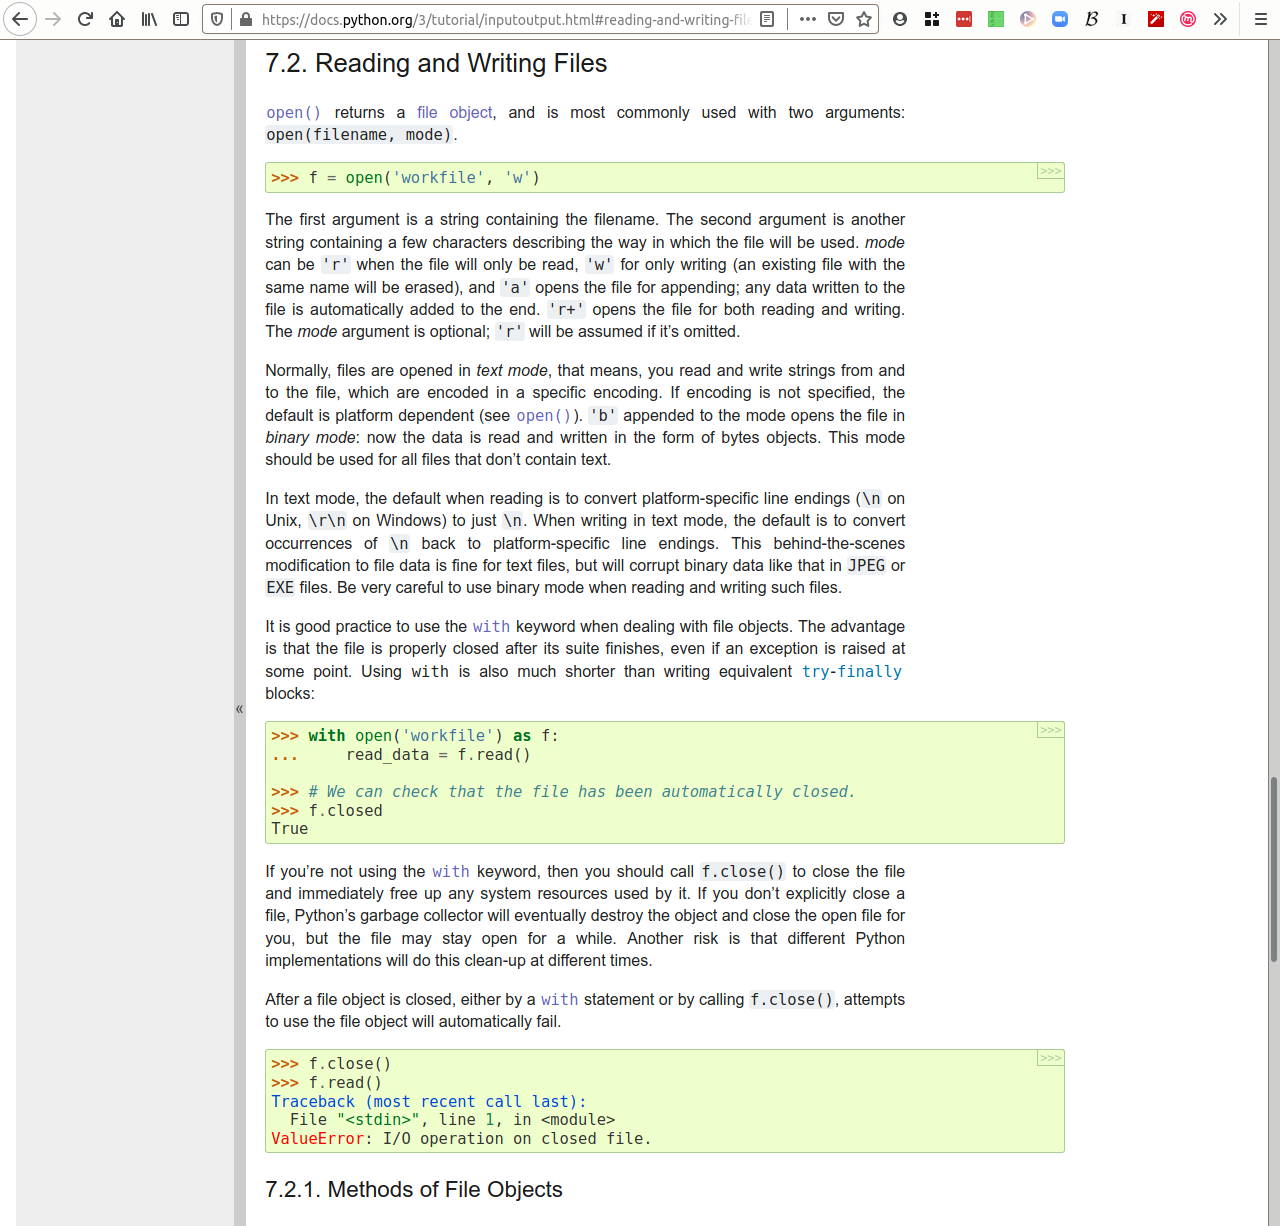
\includegraphics[width=\columnwidth]{figs/docs-files.png}
\end{frame}

\subsection{Öppna och stänga}

\begin{frame}[fragile]
  \begin{minted}[numbers=none,fontsize=\Large]{python}
file = open("filename", "r")
print(file.read())
file.close()
  \end{minted}
\end{frame}

\begin{frame}[fragile]
  \begin{example}[open\textunderscore close.py, del 1]
    \inputminted[firstline=3,lastline=16,firstnumber=3]{python}{examples/open_close.py}
  \end{example}
\end{frame}

%\begin{frame}
%  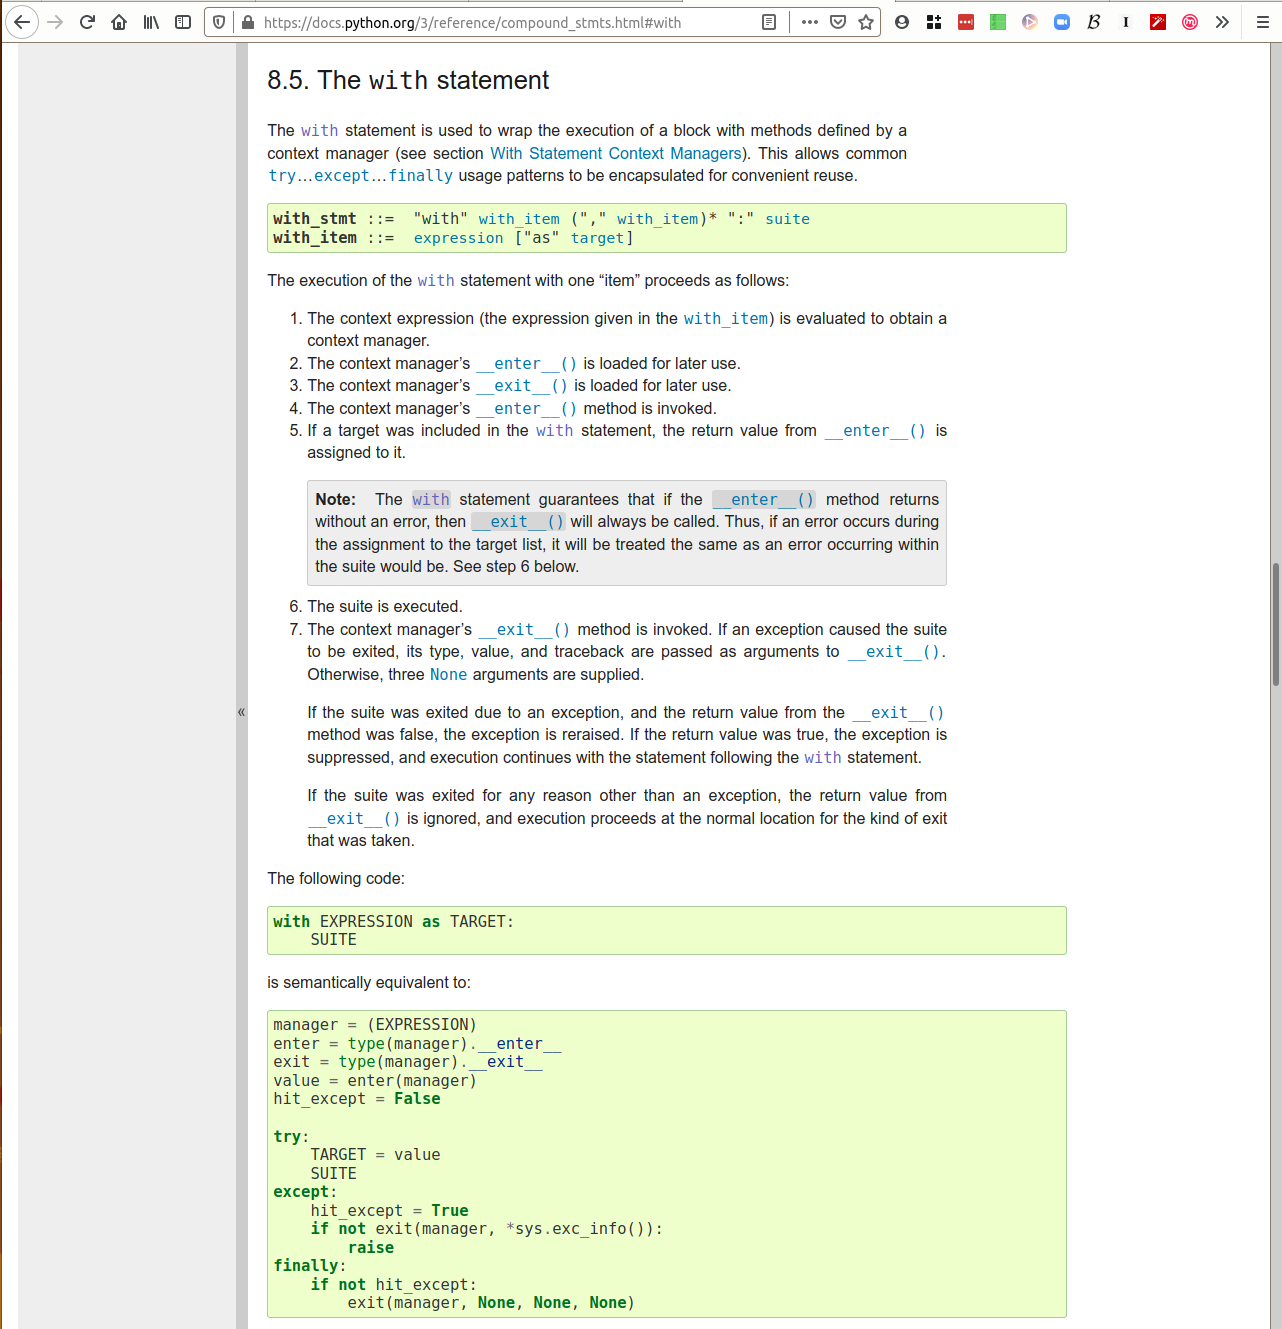
\includegraphics[width=\columnwidth]{figs/docs-with.png}
%\end{frame}

\begin{frame}[fragile]
  \begin{minted}[numbers=none,fontsize=\Large]{python}
with open("filename", "r") as file:
  print(file.read())
  \end{minted}
\end{frame}

\begin{frame}[fragile]
  \begin{example}[open\textunderscore close.py, del 2]
    \inputminted[firstline=17,lastline=27,firstnumber=17]{python}{examples/open_close.py}
  \end{example}
\end{frame}

\subsection{Läsa och skriva}

\begin{frame}[fragile]
  \begin{example}<+->[write\textunderscore file.py]
    \inputminted[firstline=5,lastline=9,firstnumber=5]{python}{examples/write_file.py}
  \end{example}

  \begin{example}<+->[read\textunderscore file.py]
    \inputminted[firstline=5,lastline=11,firstnumber=5]{python}{examples/read_file.py}
  \end{example}
\end{frame}

\begin{frame}[fragile]
  \begin{example}<+->[write\textunderscore file.py]
    \inputminted[firstline=5,lastline=9,firstnumber=5]{python}{examples/write_file.py}
  \end{example}

  \begin{example}[read\textunderscore file.py]
    \inputminted[firstline=16,lastline=20,firstnumber=5,highlightlines={7-8}]{python}{examples/read_file.py}
  \end{example}
\end{frame}

\begin{frame}[fragile]
  \begin{example}<+->[read\textunderscore file.py]
    \inputminted[firstline=5,lastline=11,firstnumber=5,highlightlines={7-10}]{python}{examples/read_file.py}
  \end{example}

  \begin{example}[read\textunderscore file.py]
    \inputminted[firstline=16,lastline=20,firstnumber=5,highlightlines={7-8}]{python}{examples/read_file.py}
  \end{example}
\end{frame}

\begin{frame}[fragile]
  \begin{example}<+->[write\textunderscore file.py]
    \inputminted[firstline=5,lastline=9,firstnumber=5,highlightlines=8]{python}{examples/write_file.py}
  \end{example}

  \begin{example}<+->[write\textunderscore file.py]
    \inputminted[firstline=14,lastline=18,firstnumber=5,highlightlines=8]{python}{examples/write_file.py}
  \end{example}
\end{frame}

\subsection{Typer av filer}

\begin{frame}
  \begin{remark}[Två typer av filer]
    \begin{description}
      \item[Textfiler] Antar \enquote{läsbara tecken}, rader bryts med 
        \mintinline{python}{'\n'}.
      \item[Binärfiler] Ingen struktur.
    \end{description}
  \end{remark}
\end{frame}

\begin{frame}
  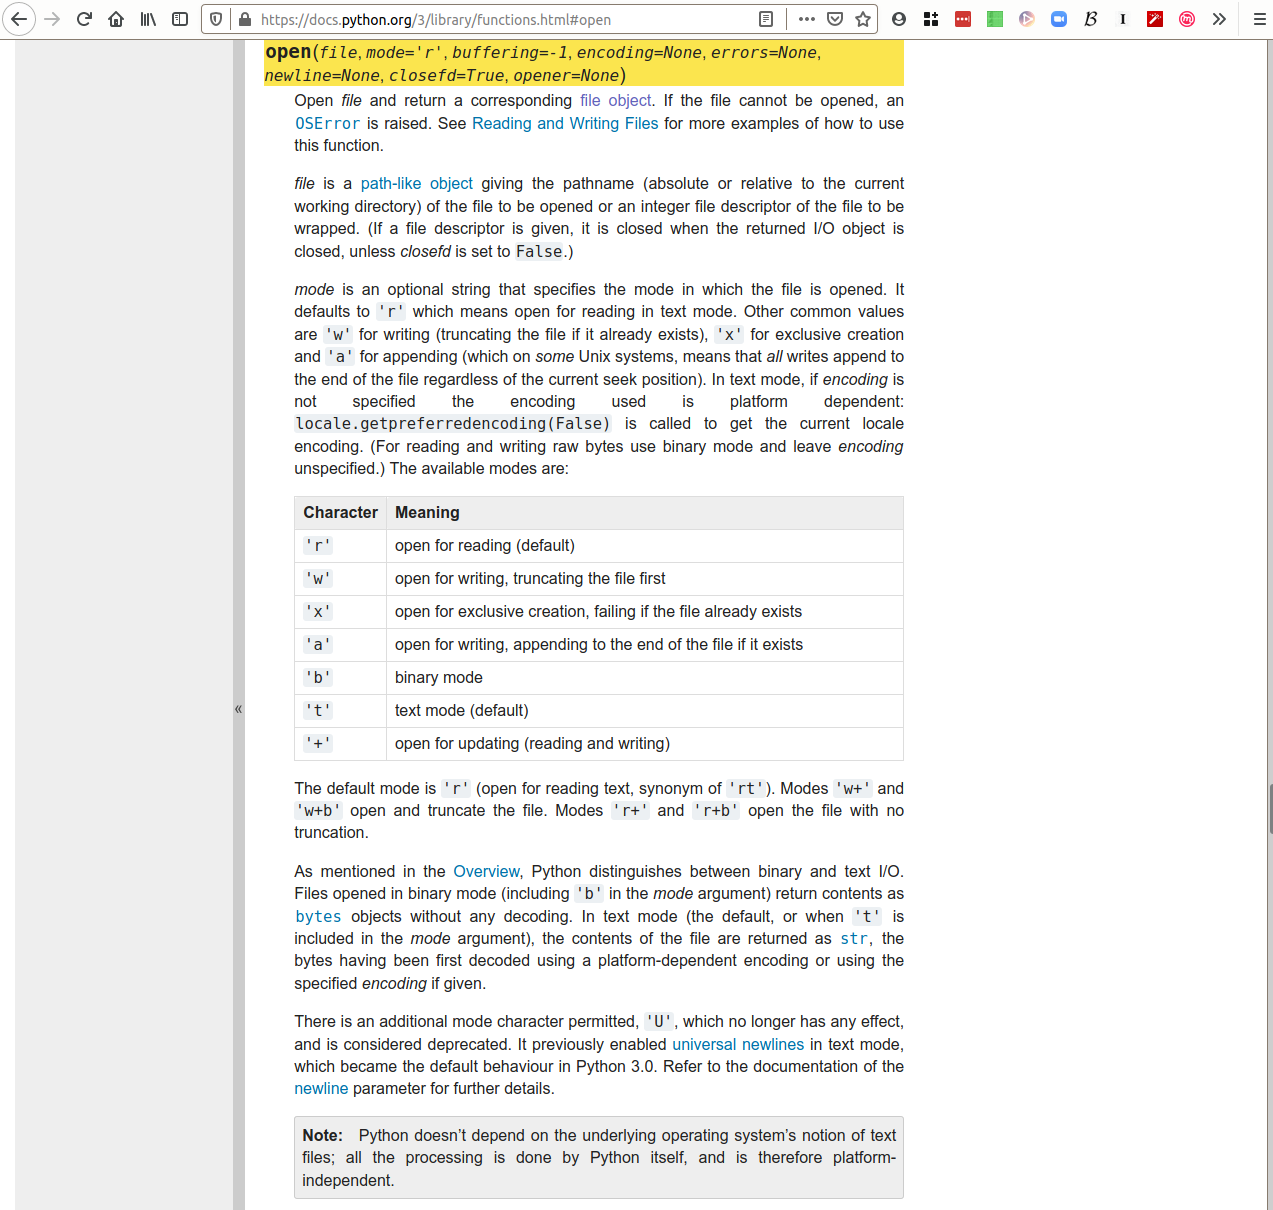
\includegraphics[width=\columnwidth]{figs/docs-open.png}
\end{frame}


\section{Filformat}

\begin{frame}[fragile]
  \begin{remark}
    \begin{itemize}
      \item Att läsa från filer är som att gå i bäcksvarta mörkret.
      \item Vi måste veta exakt var alla saker finns.
    \end{itemize}
  \end{remark}
\end{frame}

\begin{frame}
  \begin{exercise}[SCB\footnote{Idé: Olle Bälter}]
    \begin{itemize}
      \item SCB Namnsök\footnote{%
          URL: \url{https://www.scb.se/hitta-statistik/sverige-i-siffror/namnsok/}
        }
      \item Ladda ner statistikfilen.
      \item Skriv ett program som gör samma sak som webbsidans funktionalitet.
    \end{itemize}
  \end{exercise}
\end{frame}

\subsection{Egna filformat}

\begin{frame}[fragile]
  \begin{example}[xy.py]
    \inputminted[firstline=3,lastline=10,firstnumber=3]{python}{examples/xy.py}
  \end{example}
\end{frame}

\begin{frame}[fragile]
  \begin{example}[xy.py]
    \inputminted[firstline=12,lastline=26,firstnumber=12]{python}{examples/xy.py}
  \end{example}
\end{frame}

\subsection{Mer komplexa standarder}

\begin{frame}
  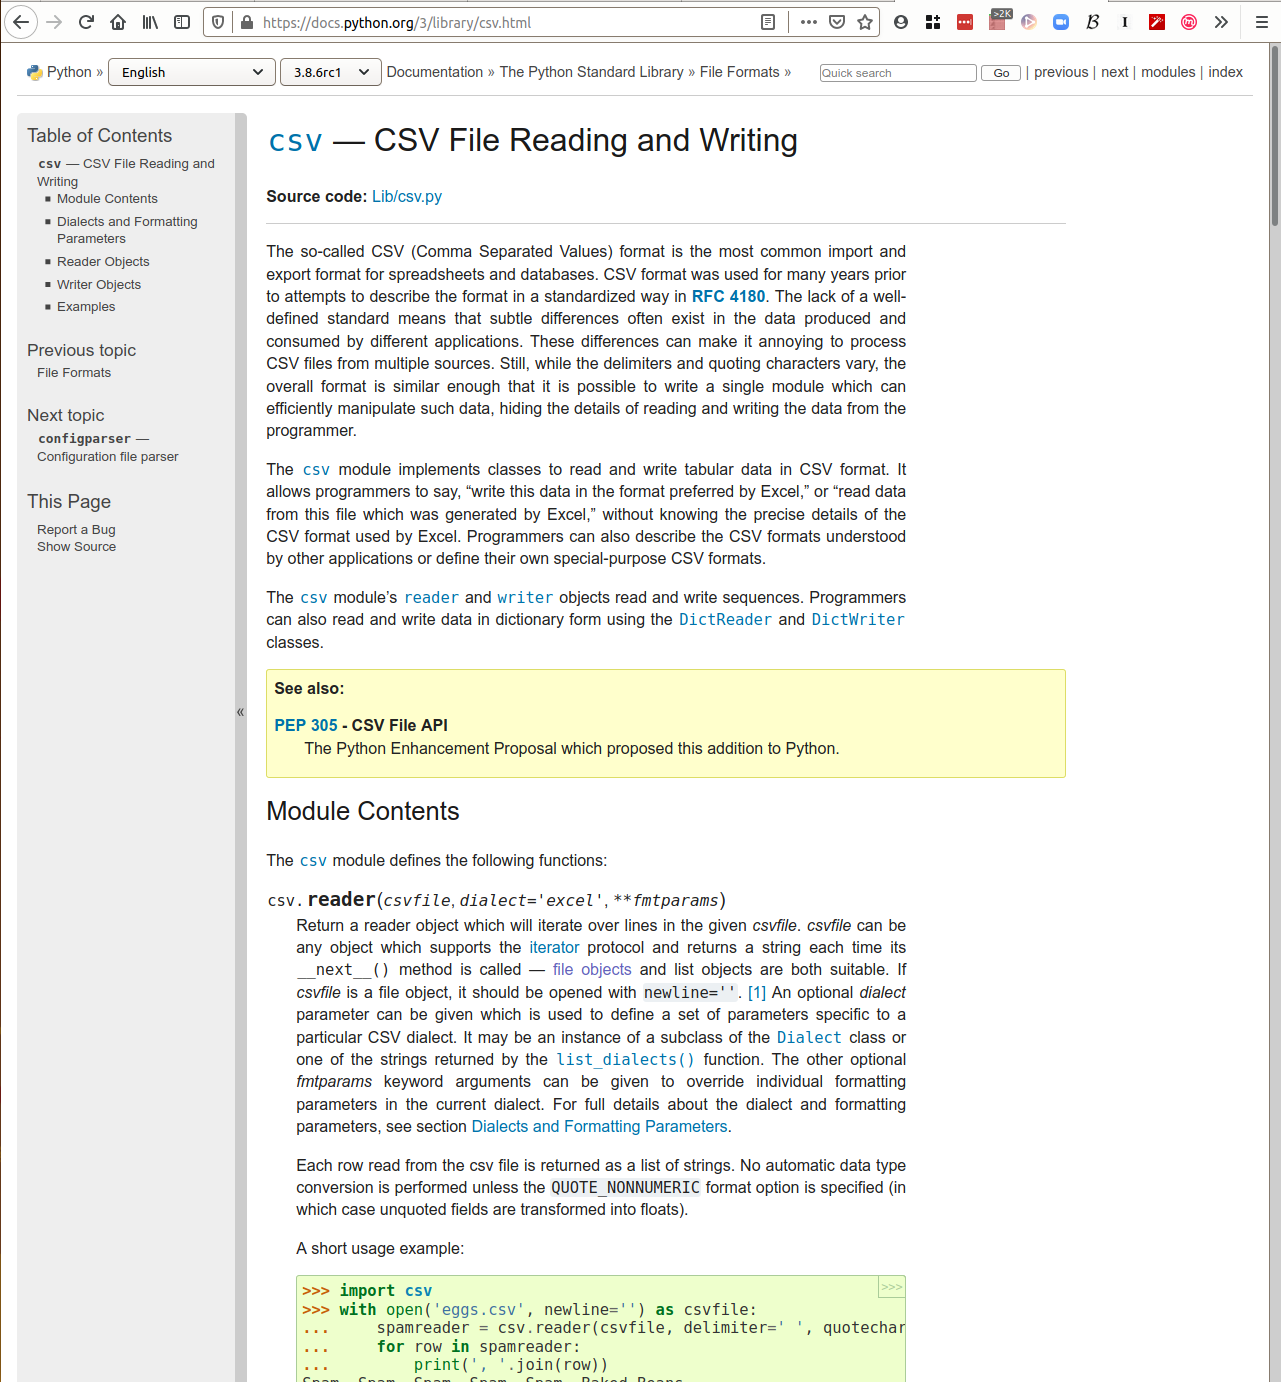
\includegraphics[width=\columnwidth]{figs/docs-csv.png}
\end{frame}

\begin{frame}[fragile]
  \begin{example}[xy\textunderscore csv.py]
    \inputminted[firstline=3,lastline=13,firstnumber=3,highlightlines={3,11,13}]{python}{examples/xy_csv.py}
  \end{example}
\end{frame}

\begin{frame}[fragile]
  \begin{example}[xy\textunderscore csv.py]
    \inputminted[firstline=15,lastline=26,firstnumber=15,highlightlines={18,20}]{python}{examples/xy_csv.py}
  \end{example}
\end{frame}
